\chapter{Pairwise Graph Convolutional Networks for Interface Prediction}
\label{chap:methods}

The methods presented in this thesis were motivated by a desire to exploit the local structure around a residue when performing interface prediction.
The biological reasoning for this is that a residue's neighborhood influences its propensity to participate in an interface.
It was noted in Chapter \ref{chap:neuralnetworks} that convolutional neural networks are one way of detecting features in a local neighborhood, but they are limited to regular grids. 
Unfortunately, proteins cannot naturally be represented as a regular grid, so convolution must be developed for a more natural representation: graphs.


\section{Proteins As Graphs}

An undirected, unweighted graph $G$ consists of a set of vertices, $V=\{v_1, v_2, ..., v_n\}$, and a set of eges, $E=\{e_1, e_2, ..., e_m\}$ where each edge is incident to two vertices and there is at most one edge between two vertices.
One way of representing proteins as graphs is to let each vertex represent a residue in the protein, and each edge represent the relationship between two residues.
Thus any information pertaining to a particular residue can be associated with the relevant vertex in the form of a feature vector.
The features used in this work are drawn from features used in prior interface prediction work \cite{minhas2014}.
Likewise, any information about the relationship between two residues can be associated with the relevant edge.
The edge features used here describe the distance between and relative orientation of two residues.
These edge features are defined between any two residues in the protein, so the graph is complete. 
A detailed explanation of each feature is contained in Appendix \ref{appendix:features}.

This representation is an abstraction of the original protein to a well studied mathematical object, with two notable facts.
First, the graph itself does not rely on a coordinate system, as is the case when working with raw 3D positions.
Second, the features contained on the graph are also not tied to a coordinate system.
This is because they either describe coordinate free attributes of individual residues, or they describe relative spatial relationships between two residues.
These facts make a protein graph invariant to rotations or translations in space.
However, since the graph was constructed from points in 3D space, local neighborhoods of vertices can be defined using spatial proximity.
This is useful when designing convolutions that use a local neighborhood as a receptive field.
We now turn our attention to graph convolution

\section{Graph Convolution}
Recent years have seen increased attention to problems involving graph structured data, prompting developments in graph convolution to perform various tasks on those data~\cite{bronstein2016}.
These developments allow leveraging of deep learning techniques, which have shown great success for problems on regular grids.
Though each variant of graph convolution is tailored to suit the data and problem being addressed, there are some common approaches which merit describing generally.
These approaches generally fall into two categories: \emph{spectral} and \emph{spatial}.


\subsection{Spectral and Spatial Graph Convolution}
Spectral methods of graph convolution are based on linear functions in the frequency domain of a graph, defined using the laplacian operator $\mathcal{L}=I-D^{-1/2}WD^{-1/2}$, where $I$ is the identity matrix, $W$ is a matrix of edge weights, and $D$ is a diagonal matrix containing the degree of each vertex~\cite{bruna2013, henaff2015, kipf2016}.
Each filter in a spectral convolution implies a weighting of each frequency in the spectral decomposition of the graph~\cite{mallat2009}.
In physics, the Laplacian operator is used to model the process of diffusion.
In a similar way, the graph Laplacian can be thought of as modeling diffusion along the edges of the graph.

Spatial approaches instead directly model the diffusion process through a transition matrix, or by defining operations in a localized neighborhood of a central vertex~\cite{henaff2015, atwood2016}.
In the latter, each neighborhood constitutes a receptive field where a convolution operation is performed (see Figure \ref{fig:spatial_graph_conv}).
Spatial convolution commonly involves a vector of weights and takes a weighted sum of neighbors, much like a discrete convolution on a grid can be viewed as taking a weighted sum of pixels within the receptive field.
Spatial convolution is more directly analogous to grid based convolution as described in Chapter \ref{chap:neuralnetworks}.
There is a critical difference, however, in that receptive fields from different parts of a graph have no natural correspondence with one another.

\begin{figure}
	\centering
	%\begin{center}
	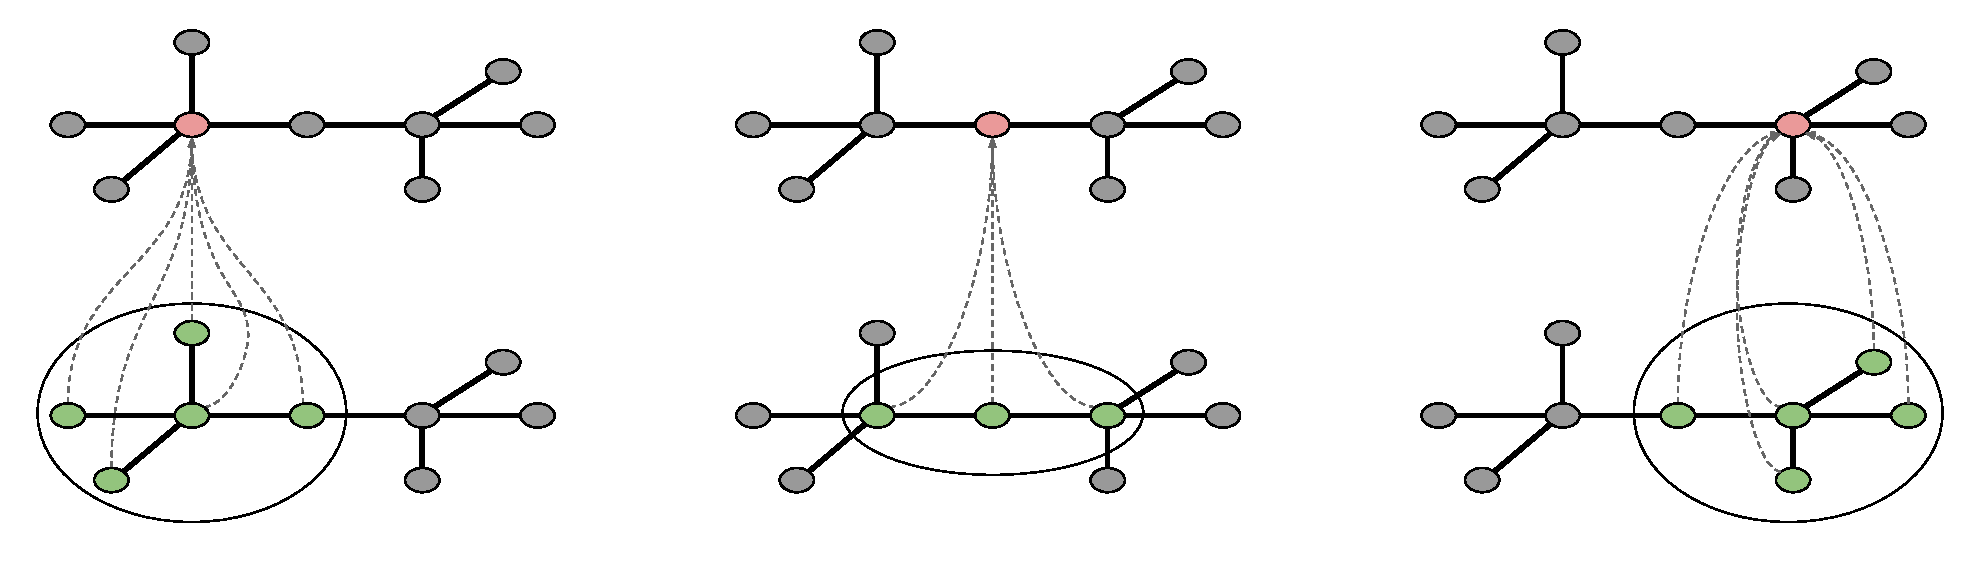
\includegraphics[width=\textwidth]{conv_graph.pdf}
	%\end{center}
	\caption{Receptive fields in a graph context, where each receptive field is defined around a central vertex. The result of convolution is applied to the central vertex in the receptive field.}
	\label{fig:spatial_graph_conv}
\end{figure}

\subsection{Receptive Field Correspondence in Spatial Convolution}


Grid receptive fields have defined positions, such as "upper left most" or "bottom middle".
Therefore weights can be applied consistently across receptive fields such that each weight is always applied to the same position.
With graphs, there is often no such correspondence between receptive fields, since vertices are inherently unordered and lack a specific position (recall their coordinate free nature).
The only well defined position is the center, but the problem persists in the neighbors.
See Figure \ref{fig:grid_vs_graph_rf}
In fact, even the number of neighbors may vary from one receptive field to another, depending on the definition of a local neighborhood.
Hence the consistent application of weights across receptive fields is only possible after these issues have been addressed.
This is typically done in one of two ways:

\begin{figure}
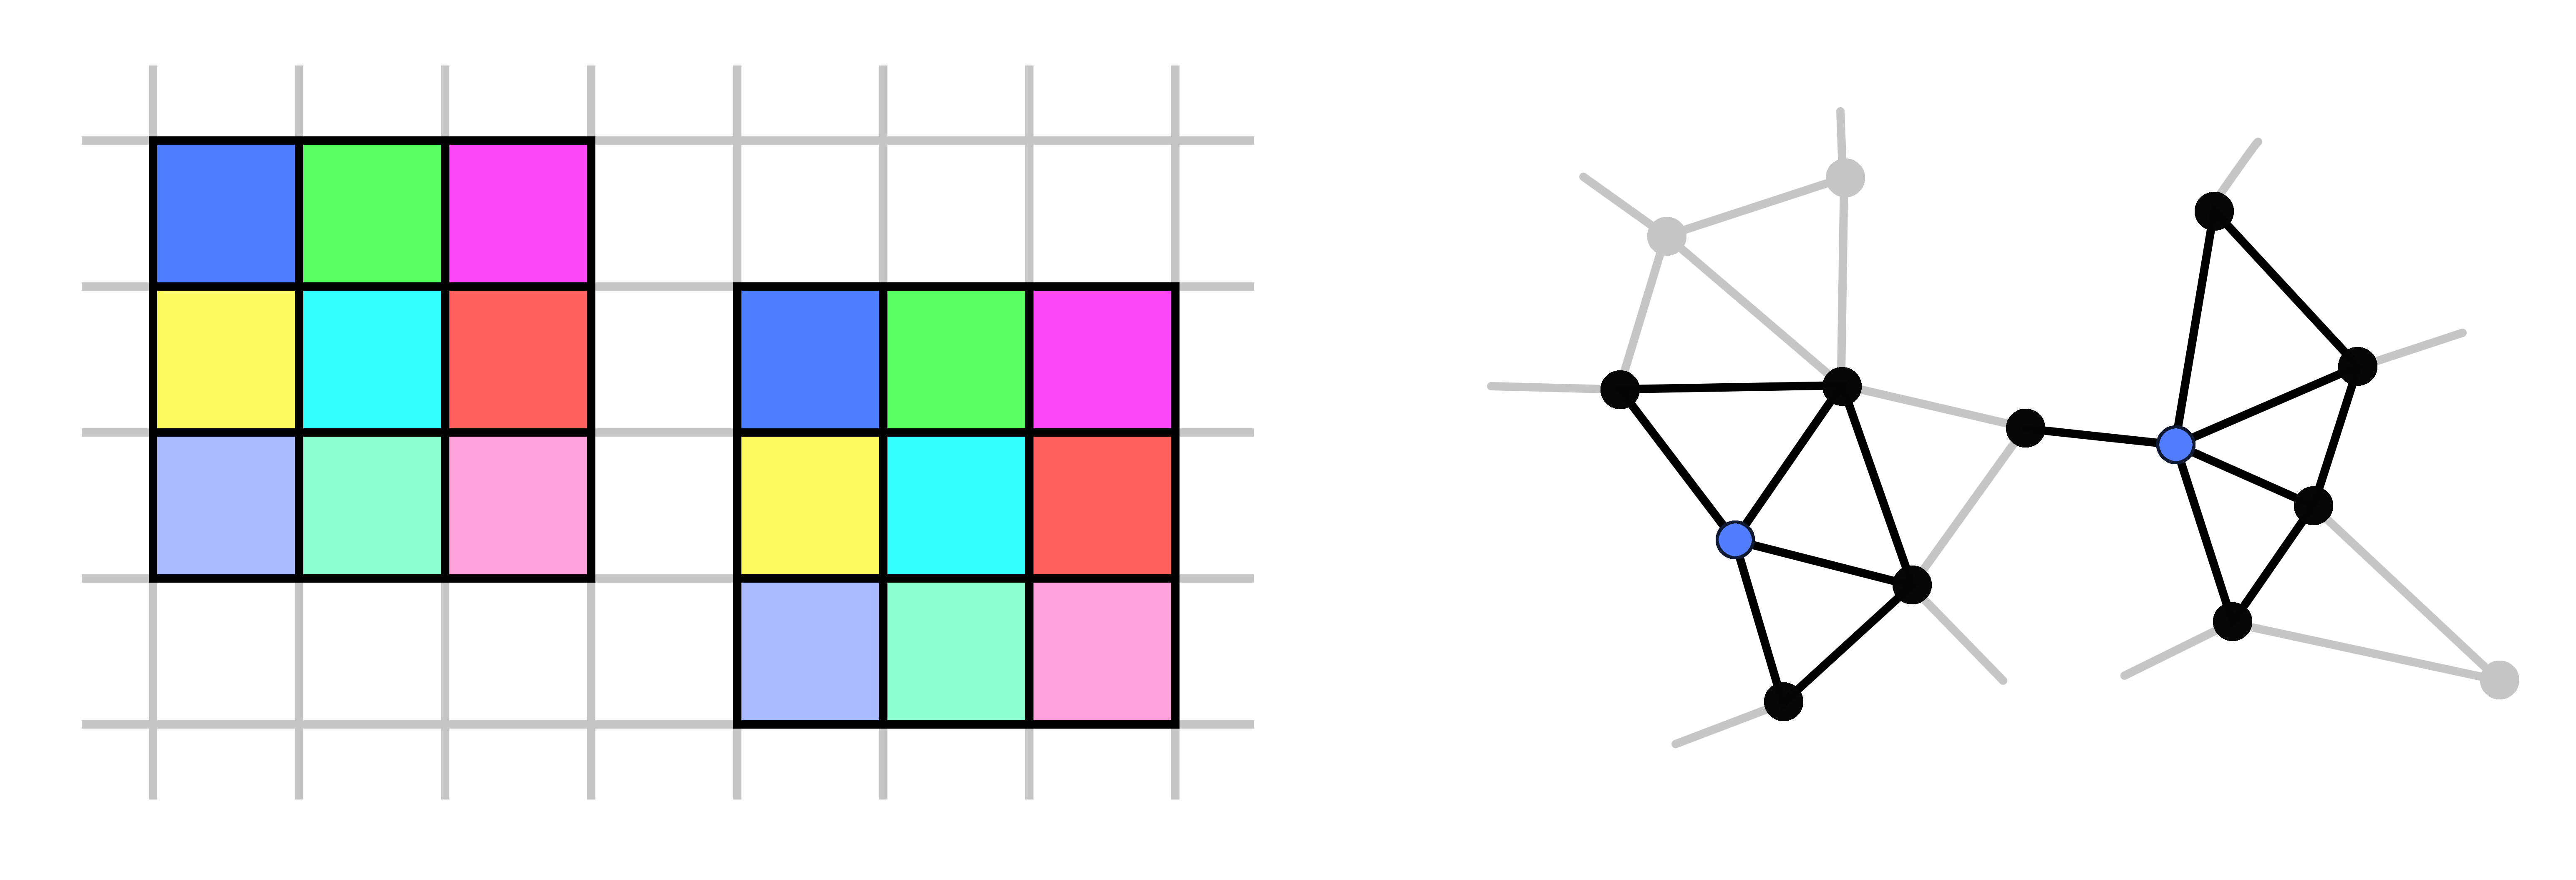
\includegraphics[width=0.9\textwidth]{grid_vs_graph_rf.png}
\caption{The difference between grid receptive fields and graph receptive fields with respect to correspondence. Grid receptive fields give rise to positions (denoted by color) which are consistent from one receptive field to another. Graphs have no positions other than the central vertex (in blue).}
\label{fig:grid_vs_graph_rf}
\end{figure}

\begin{enumerate}
	\item \emph{Imposed ordering of neighbors}. This approach establishes a correspondence between two receptive fields by ordering the neighbors in each and associating neighbors that share a common position. 
	Ordering methods are either based on vertex characteristics, like degree and betweenness centrality, or domain specific knowledge ~\cite{niepert2016, duvenaud2015}.
	They typically require the number of neighbors in a receptive field to remain the same.
	This approach allows filter weights which are applied to a particular position in the ordering, which, it is assumed, has some significance across all receptive fields.
	If the imposed ordering is arbitrary, this approach has limited utility.
	Methods following this approach can be called \emph{ordered}.
	
	\item \emph{Identical treatment of neighbors}. This approach ignores the need to establish a correspondence between receptive fields and instead treats all neighbors identically.
	Rather than apply different weights to neighbors depending on their position in an ordering, the same weights are applied to each neighbor.
	This allows for different sizes of receptive fields and avoids choosing an ordering method, but lacks the ability to treat each neighbor uniquely.
	Methods following this approach can be called \emph{order-free}.
\end{enumerate}

Figure \ref{fig:correspondence_approaches} depicts both approaches.
Examples of each were evaluated for this thesis.
In addition, proposed convolutions were examined which attempt to incorporate the advantages of both ordered and order-free methods.
Below is a description of each existing method followed by the proposed methods presented in this thesis. 

\begin{figure}
	\centering
	%\begin{center}
	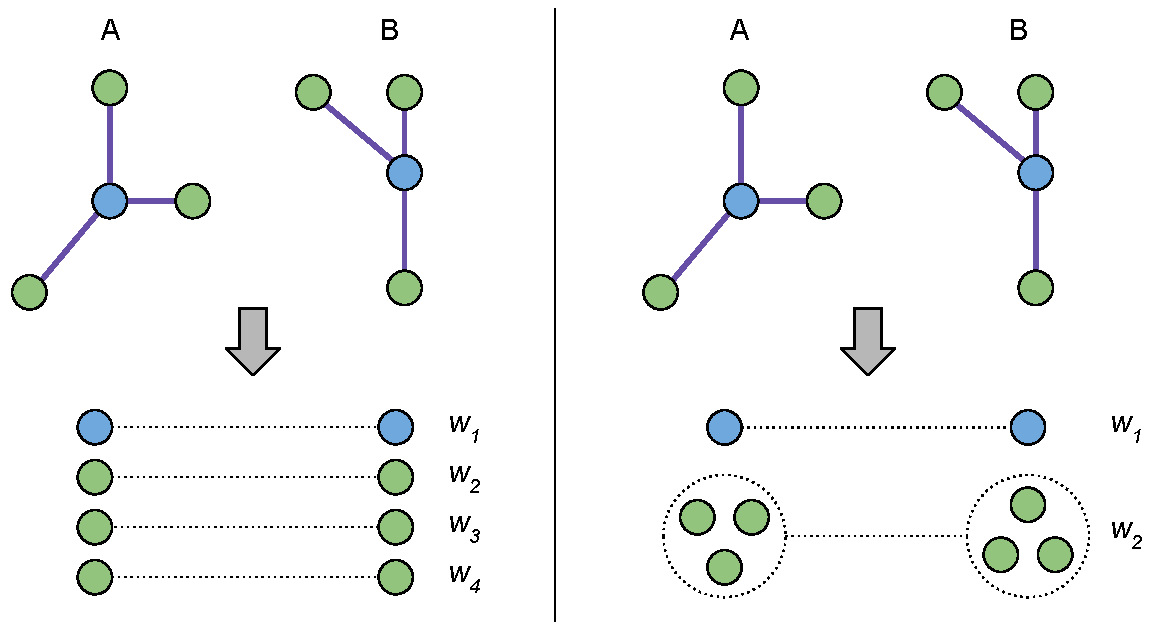
\includegraphics[width=0.8\textwidth]{correspondence_approaches.pdf}
	%\end{center}
	\caption{Two approaches of establishing correspondence between the neighbors of receptive fields A and B. Central vertices are shown in blue and neighbors in green. The central vertices always correspond with one another. Left: neighbors are ordered and placed into correspondence based on position. Unique weights (\emph{$w_2$--$w_4$}) can then be applied to each position in the order. Right: neighbors are left unordered and treated identically. This requires that the same weights (\emph{$w_2$}) be used for all neighbors.}
	\label{fig:correspondence_approaches}
\end{figure}


\subsection{Diffusion Based Method}
As mentioned, spectral methods utilize the Laplacian operator, which is used to model diffusion processes. 
Although no spectral methods were examined in this thesis, a spatial diffusion method was.
Atwood \& Towsley~\cite{atwood2016} proposed a Diffusion Convolutional Neural Network (DCNN) which converts a graph's weight matrix to a transition matrix by normalizing its rows.
The transition matrix $P$ is raised to successive exponents, generating a power series, with each power corresponding to all walks of length equivalent to that power.
For a maximum power of $L$, the activation of a vertex is:

\begin{equation}
h(x_i | W) = \sigma \bigg( \sum_{l=0}^L (W_{l\cdot} \odot P^l X ) \bigg),
\label{eq:diffusion}
\end{equation}

\noindent
where $W$ is a matrix of weights, $W_{l\cdot}$ is its $l^{th}$ row, $\odot$ denotes broadcasted elementwise multiplication, and $X$ is a matrix of all vertices, where each row is a vertex and each column a different feature.
For each power $l$, all vertices that have a random walk of length $l$ that end at the vertex of interest are summed together, weighted by the walk probability.
This sum is then multiplied elementwise with a weight vector and summed with the result of all other powers to produce the overall signal.
Unlike other spatial convolutions presented in this thesis, this method does not use a receptive field, instead relying on the similarity matrix to indicate proximity.


\subsection{Ordered Method}

Niepert, Ahmed, \& Kutzkov~\cite{niepert2016} described an ordered graph convolution, \emph{PATCHY-SAN}, which performs classification at the graph level.
This method constructs local neighborhoods and orders neighboring vertices according to a \emph{normalization} procedure.
The ordered vertices serve as the receptive field for convolution at the central vertex, which is also in the ordering. 
If $(x_1, x_2, ... , x_k)$ is the ordered list of vertices, then convolution takes the form:

\begin{equation}
h(x_i | \{ W_{j} \}, b)= \sigma \bigg( \frac{1}{k} \sum_{j=1}^{k}(W_{j} x_j) + b \bigg),
\label{eq:patchysan}
\end{equation}

\noindent
where $W_j$ is the weight matrix for position $j$ in the ordering.
A natural ordering technique is one which places the central vertex first and orders its neighbors from least to greatest distance from the center. 
In this way, one weight matrix is used for all central vertices, another for all nearest neighbors, etc.
The vertex ordering also imposes a lexicographic ordering on the neighborhood edges as well, so unique weights can be used to generate a signal from each edge. 
Adding this term to the convolution generates:

\begin{equation}
h(x_i | \{ W_{j} \}, \{ W_{jk} \}, b)= \sigma \bigg( \frac{1}{k} \sum_{j=1}^{k}(W_{j} x_j) + \frac{1}{k^2} \sum_{j = 1}^{k-1} \sum_{l=j+1}^{k}(W_{jk} A_{jk})  + b \bigg),
\label{eq:patchysan_2e}
\end{equation}

\noindent
where $W_{jl}$ is the weight matrix associated with edge $(j, l)$ in the lexicographic ordering, and $A_{jk}$ is the feature vector associated with edge $(j, k)$.
Originally, Niepert et al. convolved vertices and edges separately and combine them in a subsequent layer.
Classification is then performed on the whole graph level.
For interface prediction however, the edges and vertex signals are averaged together and applied to the central vertex so that repeated graph convolutions may be performed without losing the graph structure.


\subsection{Order-Free Methods}
One of the simplest forms of order-free graph convolution was proposed by Duvenaud \& Maclaurin, et al.~\cite{duvenaud2015}, which was used for generating molecular \emph{fingerprints}.
This method uses a single set of weights for all vertices in the receptive field, including the central vertex:

\begin{equation}
h(x_i | W, b)= \sigma \bigg( W x_i +  \frac{1}{|\mathcal{N}_i|} \sum_{j \in \mathcal{N}_i} (W x_j) + b\bigg),
\label{eq:fingerprint}
\end{equation}

\noindent
where $\mathcal{N}_i$ is the index set of all neighbors of $x_i$.
In the original formulation, no bias term was included, and the sum was not divided by the neighborhood size.
However, when used for interface prediction, including the bias and normalization provided better overall results.

As mentioned, center vertices may be treated separately from the neighbors, even if all neighbors are treated identically. 
Schlichtkrull \& Kipf~\cite{schlichtkrull2017} proposed such an approach called \emph{Relational Graph Convolutional Networks}, or R-GCN.
Their methods were developed for use in knowledge bases, graph structures where the vertices are named entities and the edges capture the many binary relationships between the entities. 
To convolve a vertex, they take the neighborhood defined by each relation type and sum the signal from all the neighbors in that neighborhood.
The resultant signal is the sum of signals from each relation type.
For protein graphs, spatial proximity is the only method for determining neighborhoods that makes sense biologically, so there is only one neighborhood.
The adapted version of this convolution for use in interface prediction is:

\begin{equation}
h(x_i | W^\textsc{c}, W^\textsc{n}, b)= \sigma \bigg( W^\textsc{c} x_i + \frac{1}{|\mathcal{N}_i|} \sum_{j \in \mathcal{N}_i}(W^\textsc{n} x_j)  + b\bigg),
\label{eq:rgcn}
\end{equation}

\noindent
where separate weight matrices, $W^\textsc{c}$ and $W^\textsc{n}$, are used for the center and neighbors, respectively
In the original version, a different weight matrix was used for each of the many relation types.  
To tie learning across all relation types, all weight matrices were simply linear combinations of a set of learnable basis weight matrices:

\begin{equation}
\begin{split}
W^\textsc{n} = \sum_{b} a^\textsc{n}_b V_b \\
W^\textsc{c} = \sum_{b} a^\textsc{c}_b V_b 
\end{split}
\label{eq:rgcn_basis}
\end{equation}

\noindent
where $\{V_b\}$ is a set of basis matrices, and $a^\textsc{c}$ and $a^\textsc{n}$ are scalar weights that combine the basis matrices to create $W^\textsc{c}$ and $W^\textsc{n}$, respectively.
For interface prediction, R-GCNs were examined both with and without basis matrices.

The above order-free methods do not incorporate edge information.
Sch{\"u}tt, Arbabzadah, Chmiela, M{\"u}ller, \& Tkatchenko~\cite{schutt2017} proposed a version called \emph{Deep Tensor Neural Networks} (DTNN) which creates a signal for the neighbor vertices as well as the edges which connect them to the central vertex:

\begin{equation}
h(x_i | W, W^\textsc{n}, W^\textsc{e}, b^\textsc{n}, b^\textsc{e})= x_i + \frac{1}{|\mathcal{N}_i|} \sum_{j \in \mathcal{N}_i} \sigma \bigg[ W \bigg( (W^\textsc{n} x_j + b^\textsc{n}) \odot (W^\textsc{e} A_{ij} + b^\textsc{e}) \bigg) \bigg],
\label{eq:deep_tensor}
\end{equation}

\noindent
where $\odot$ denotes the elementwise product.
In this formulation, $W^\textsc{n}$ and $W^\textsc{e}$ transform vertices and edges respectively into a common space, and $W$ transforms their combination to have the same dimensionality as the input. 
This convolution does not transform the input by any weight matrix, rather it can be viewed as updating the representation at $x_i$ using information from its neighbors.
This restricts representations to always have the same dimensionality, which is not generally required in convolutions. 
Again, the normalization is omitted from the original formulation, but consistently improves performance when performing interface prediction.
Nevertheless, this method uniquely incorporates edge information, so that even while all neighbors use the same weight matrix, the information on their edges is used to differentiate them.
This concept is carried forward into the convolution methods proposed below.


\subsection{Proposed Order-Free Methods}
Like DTNN, these methods incorporate edge information to help differentiate neighbors, but also avoid imposing an arbitrary ordering on the neighbors in a receptive field.
This is accomplished by incorporating information from the edges between each neighbor and the central vertex.
Here are two variants of graph convolution which differ only in how the edge information is incorporated, denoted \emph{Sum Coupling} and \emph{Product Coupling}.
For a central vertex $i$ on the graph and a local neighborhood of vertices $\mathcal{N}_i$, the output of Sum Coupling graph convolution is:
\begin{equation}
h(x_i | W^\textsc{c}, W^\textsc{n}, W^\textsc{e}, b) = \sigma \bigg( W^{\textsc{c}} x_i + \frac{1}{|\mathcal{N}_i|}\sum_{j \in \mathcal{N}_i} (W^{\textsc{n}} x_j + W^{\textsc{e}} A_{ij}) + b \bigg),
\label{eq:sum_coupling}
\end{equation}
where $x_i$ is the feature vector associated with vertex $i$, $W^\textsc{c}$, $W^\textsc{n}$ and $W^\textsc{e}$ are weight matrices, and $b$ is a vector of biases. 
Intuitively, this calculates an activation for the central vertex, each neighbor vertex, and each edge between a neighbor and the central vertex separately.
It is the inclusion of edge activations that allows each neighbor to be distinguished from the others on the basis of its relationship to the central vertex.
This variant is called Sum Coupling because the neighbor vertex and edge activations are added together.
Because of this, the direct association between a neighbor its edge is lost.
A variant which maintains the association is Product Coupling, which output is:
\begin{equation}
h(x_i | W^\textsc{c}, W^\textsc{n}, W^\textsc{e}, b) = \sigma \bigg( W^{\textsc{c}} x_i + \frac{1}{|\mathcal{N}_i|}\sum_{j \in \mathcal{N}_i} (W^{\textsc{n}} x_j \odot W^{\textsc{e}} A_{ij}) + b \bigg),
\label{eq:prod_coupling}
\end{equation}
where $\odot$ denotes the elementwise product between two vectors or matrices. 
This allows a neighbor's influence on the overall activation to be modulated by its relationship to the central vertex.
For protein graphs, this means neighboring residues will contribute more or less to the overall activation, depending on their distance from and relative orientation to the central vertex, with the precise modulation determined by the edge activations.

In relation to prior methods, Sum Coupling is most similar to Fingerprint and R-GCN convolutions.
Unlike Fingerprint convolutions, it uses separate weights for central and neighbor vertices.
Unlike R-GCN convolutions, it does not use basis functions which tie together all weight matrices.
Also, Fingerprint and R-GCN convolutions do not generate signals from the edges.
Product Coupling is similar to DTNN convolutions in the way vertex and edge information is coupled together, but unlike DTNN it calculates a signal for the central vertex and allows the number of channels/features to change layer by layer. 

The receptive fields are always defined around a central vertex, so the results of convolution can be applied to that vertex.
This retains the graph structure after each convolution, so convolutional layers are stackable, just like convolutions on grids.

A note on receptive fields: protein graphs are complete and embedded in a metric space, so we can define a receptive field using a fixed number of closest neighbors to the central vertex.
A receptive field can also be defined using a threshold $\delta>0$ such that all vertices closer to the central vertex than the threshold are included in the receptive field.
All neighbors in a receptive field are guaranteed to share an edge with the central vertex, allowing the application of equations (\ref{eq:sum_coupling}) and (\ref{eq:prod_coupling}).
For incomplete graphs, a receptive field can be defined as all vertices within $k$ hops of the central vertex. 
If $k=1$, both Sum and Product Coupling can directly be applied.
If $k>1$, then Product Coupling can't be directly applied to neighbors more than 1 hop away from the center vertex, since they share no edge with the center. 
Though there are ways to deal with this issue, they are not the focus of this thesis.

Lastly, to assess the benefit that incorporating information from neighboring residues has on classification performance, the \emph{No Convolution} variant is defined as:

\begin{equation}
h(x_i | W^\textsc{c}, b)= \sigma \bigg( W^{\textsc{c}} x_i + b \bigg),
\label{eq:no_conv}
\end{equation}

\noindent
which excludes all neighbors.
Note the similarity to Equation (), except that in this case the output is just for a single vertex rather than for the entire layer.


\section{Pairwise Neural Network Architecture}
These graph convolution operations allow the detection of local patterns on a single graph, and produce a new representation at each vertex.
Partner specific protein interaction, however, requires classifying pairs of residues in different proteins (vertices in different graphs), which is equivalent to making predictions on vertices in the product graph. 
Such predictions are made using a pairwise neural network architecture.

A pairwise architecture consists first of two identical convolutional modules, each responsible for generating the representation for one of the proteins in the pair.
A key requirement for the pairwise architecture is symmetry, since the prediction for a pair of residues should be the same irrespective of which leg is used for which protein.
To ensure symmetry in the convolution layers, weights are shared between layers in the different modules.
The merge layer then combines the vertex representations from one graph with the vertex representations from the other into pairs.
To maintain symmetry, this merge process should also be symmetric.
For example, the elementwise sum, elementwise product, and outer-product are all commutative and therefore produce symmetric output.
Another option is to combine pairs asymmetrically (e.g. concatenate the two representations together), but then average the predictions from each ordering of the pair.
Finally, the combined representation for each pair of residues is passed through a number of fully connected layers.
The data are represented as pairs of residues at this point. 
Theoretically, graph convolution could be performed at this stage as well, this time in the product graph.
However, the computational and memory requirements of doing so prove prohibitive, since the number of convolutions and the number of neighbors in each convolution increases quadratically in the graph size.
Hence the work in this thesis performs no convolution after merging.
The final layer has a single output for each pair indicating the prediction for that pair.
See Figure \ref{fig:pairwise_arch1} for a graphical depiction.

This output is converted to a binary class prediction vector using a softmax function, 

\begin{equation}
\text{softmax}(x) = \bigg[ \frac{e^{-x}}{e^{x} + e^{-x}} , \frac{e^{x}}{e^{x} + e^{-x}} \bigg],
\label{eq:softmax}
\end{equation}

\noindent
the elements of which can be interpreted as class probabilities for the negative (non-interfacial) and positive (interfacial) classes, respectively.
This output is compared to a one-hot label vector indicating whether \big($[0, 1]$\big) or not\big($[1, 0]$\big) the pair constitute part of the true interface. 

\begin{figure}
	\includegraphics[width=\textwidth]{pairwise_network4.pdf}
	\caption{A pairwise neural network architecture that takes two protein graphs as input. Each leg contains one or more convolutional layers. The resultant graphs are then merged to create representations of residue pairs. After more fully connected layers, a final classification is performed for each pair.}
	\label{fig:pairwise_arch1}
\end{figure}


This chapter has presented protein graphs, graph convolution operations, and pairwise neural network architectures, all of which are components in this thesis' approach to partner specific protein interface prediction.
Chapter \ref{chap:experiments} describes the experiments that were performed.
